\documentclass[../../main.tex]{subfiles}

\graphicspath{{../../image/}{../../figure/}}

\begin{document}

\section{习题}\label{section:ch02-习题}

\begin{exercise}\label{exercise:ch02-01}
（$\bigstar$）在癌症检查的示例中，我们使用了癌症的先验概率 $p(C=1)=0.01$。实际上，癌症的流行程度通常要低得多。考虑 $p(C=1)=0.001$ 的情况，并重新计算在检查结果为阳性的情况下某人患有癌症的概率 $p(C=1\mid T=1)$。结果可能会让许多人感到惊讶，因为检查似乎具有很高的准确性，但检查结果呈阳性情况下患有癌症的概率却很低。
\end{exercise}

\begin{exercise}\label{exercise:ch02-02}
（$\bigstar\bigstar$）确定的数满足传递性（transitivity），即如果 $x>y$ 且 $y>z$，则可以推出 $x>z$。然而，随机数不满足传递性。\cref{figure:ch02-非传递骰子}展示了 $4$ 个立方体骰子，我们规定了它们的循环顺序。请证明这 $4$ 个骰子中，每一个掷出的数字比循环中前一个骰子掷出数字大的概率为 $2/3$。这样的骰子称为非传递骰子（non-transitive dice），这里显示的具体例子称为 Efron 骰子（Efron dice）。
\end{exercise}

\begin{figure}[htbp]
  \centering
  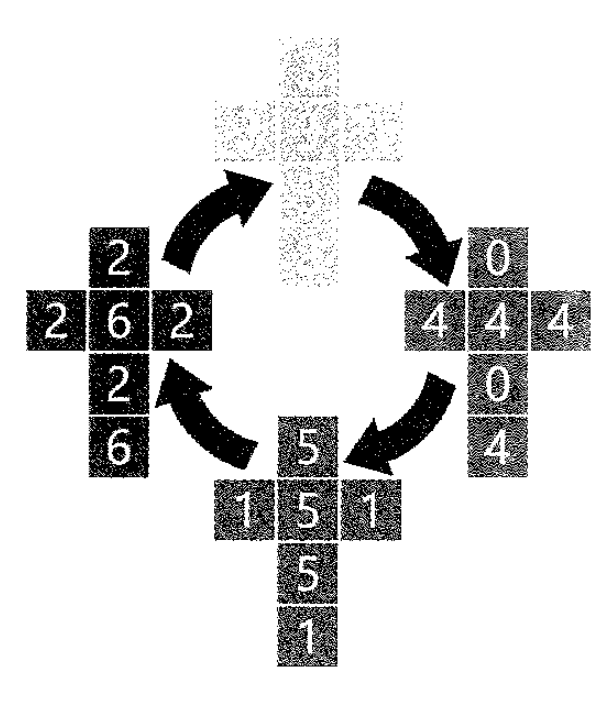
\includegraphics[width=0.42\textwidth]{ch02-fig2-16-efron-dice.png}
  \caption{非传递立方体骰子的一个示例，其中每个骰子都已被“扁平展开”以展示每个面上的数字。骰子按循环顺序排列，使得每个骰子掷出的数字比循环中前一个骰子掷出数字大的概率为 $2/3$。}
  \label{figure:ch02-非传递骰子}
\end{figure}

\begin{exercise}\label{exercise:ch02-03}
（$\bigstar$）考虑由两个独立随机变量之和给出的变量 $y=u+v$，其中 $u\sim p_u(u)$ 且 $v\sim p_v(v)$。证明 $y$ 的分布 $p_y(y)$ 可由下式给出：
\begin{align}
  p(y) = \int p_u(u)\,p_v(y-u)\,\mathrm{d}u
  \label{align:ch02-卷积}
\end{align}
这称为 $p_u(u)$ 和 $p_v(v)$ 的卷积（convolution）。
\end{exercise}

\begin{exercise}\label{exercise:ch02-04}
（$\bigstar$）验证均匀分布［\eqref{align:ch02-均匀分布}］被正确地归一化了，并找出其均值和方差的表达式。
\end{exercise}

\begin{exercise}\label{exercise:ch02-05}
（$\bigstar\bigstar$）验证指数分布［\eqref{align:ch02-指数分布}］和 Laplace 分布［\eqref{align:ch02-Laplace分布}］被正确地归一化了。
\end{exercise}

\begin{exercise}\label{exercise:ch02-06}
（$\bigstar$）利用 Dirac $\delta$ 函数的性质，验证经验密度［\eqref{align:ch02-经验分布}］被正确地归一化了。
\end{exercise}

\begin{exercise}\label{exercise:ch02-07}
（$\bigstar$）通过使用经验密度［\eqref{align:ch02-经验分布}］，证明可以对从密度中抽取的有限样本集合进行求和［\eqref{align:ch02-样本近似}］，并近似由\eqref{align:ch02-连续期望}给出的期望。
\end{exercise}

\begin{exercise}\label{exercise:ch02-08}
（$\bigstar$）使用方差定义［\eqref{align:ch02-方差}］证明 $\mathrm{var}[f(x)]$ 满足\eqref{align:ch02-方差展开}。
\end{exercise}

\begin{exercise}\label{exercise:ch02-09}
（$\bigstar$）证明如果两个变量 $x$ 和 $y$ 相互独立，则它们的协方差为零。
\end{exercise}

\begin{exercise}\label{exercise:ch02-10}
（$\bigstar$）假设两个变量 $x$ 和 $z$ 统计独立，证明它们的和的均值和方差满足
\begin{align}
  \mathbb{E}[x+z] &= \mathbb{E}[x]+\mathbb{E}[z]
  \label{align:ch02-和均值}
\end{align}
\begin{align}
  \mathrm{var}[x+z] &= \mathrm{var}[x]+\mathrm{var}[z]
  \label{align:ch02-和方差}
\end{align}
\end{exercise}

\begin{exercise}\label{exercise:ch02-11}
（$\bigstar$）考虑具有联合分布 $p(x,y)$ 的两个变量 $x$ 和 $y$。证明以下两个结论：
\begin{align}
  \mathbb{E}[x] &= \mathbb{E}_{y}\left[\mathbb{E}_{x}[x\mid y]\right]
  \label{align:ch02-全期望}
\end{align}
\begin{align}
  \mathrm{var}[x] &= \mathbb{E}_{y}\left[\mathrm{var}_{x}[x\mid y]\right] + \mathrm{var}_{y}\left[\mathbb{E}_{x}[x\mid y]\right]
  \label{align:ch02-全方差}
\end{align}
其中 $\mathbb{E}_{x}[x\mid y]$ 表示条件分布 $p(x\mid y)$ 下 $x$ 的期望，条件方差的符号同理。
\end{exercise}

\begin{exercise}\label{exercise:ch02-12}
（$\bigstar$）证明单变量 Gauss 分布的归一化条件［\eqref{align:ch02-Gauss归一化}］。为此，考虑积分
\begin{align}
  I = \int_{-\infty}^{\infty}\exp\left(-\frac{1}{2\sigma^{2}}x^{2}\right)\mathrm{d}x
  \label{align:ch02-Gauss积分}
\end{align}
首先将其平方写成以下形式：
\begin{align}
  I^{2} = \int_{-\infty}^{\infty}\!\!\int_{-\infty}^{\infty}\exp\left(-\frac{1}{2\sigma^{2}}(x^{2}+y^{2})\right)\mathrm{d}x\,\mathrm{d}y
  \label{align:ch02-Gauss积分平方}
\end{align}
然后从直角坐标 $(x,y)$ 转换到极坐标 $(r,\theta)$，并代入 $u=r^{2}$。证明通过对 $\theta$ 和 $u$ 进行积分，然后对两边取平方根，可以得到
\begin{align}
  I = \left(2\pi\sigma^{2}\right)^{1/2}
  \label{align:ch02-Gauss积分值}
\end{align}
最后，用这个结果来证明 Gauss 分布 $\mathcal{N}(x\mid\mu,\sigma^{2})$ 是归一化的。
\end{exercise}

\begin{exercise}\label{exercise:ch02-13}
（$\bigstar\bigstar$）通过改变变量，验证单变量 Gauss 分布［\eqref{align:ch02-单变量Gauss}］满足\eqref{align:ch02-Gauss均值}。接下来，对归一化条件
\begin{align}
  \int_{-\infty}^{\infty}\mathcal{N}(x\mid\mu,\sigma^{2})\,\mathrm{d}x = 1
  \label{align:ch02-归一化条件}
\end{align}
关于 $\sigma^{2}$ 微分，验证 Gauss 分布满足\eqref{align:ch02-Gauss二阶矩}。最后，证明\eqref{align:ch02-Gauss方差}成立。
\end{exercise}

\begin{exercise}\label{exercise:ch02-14}
（$\bigstar$）证明 Gauss 分布［\eqref{align:ch02-单变量Gauss}］的众数（即极大值）由 $\mu$ 给出。
\end{exercise}

\begin{exercise}\label{exercise:ch02-15}
（$\bigstar$）通过将对数似然函数［\eqref{align:ch02-对数似然}］关于 $\mu$ 和 $\mu^{2}$ 的导数置为零，验证结果\eqref{align:ch02-均值最大似然}和\eqref{align:ch02-方差最大似然}。
\end{exercise}

\begin{exercise}\label{exercise:ch02-16}
（$\bigstar\bigstar$）使用结论\eqref{align:ch02-Gauss均值}和\eqref{align:ch02-Gauss二阶矩}，证明
\begin{align}
  \mathbb{E}\left[x_nx_m\right] = \mu^{2} + I_{nm}\sigma^{2}
  \label{align:ch02-混合矩}
\end{align}
其中 $x_n$ 和 $x_m$ 表示从均值为 $\mu$ 和方差为 $\sigma^{2}$ 的 Gauss 分布中抽取的数据点，$I_{nm}$ 满足如果 $n=m$，$I_{nm}=1$，否则 $I_{nm}=0$，从而证明结论\eqref{align:ch02-均值无偏}和\eqref{align:ch02-方差有偏}。
\end{exercise}

\begin{exercise}\label{exercise:ch02-17}
（$\bigstar$）使用定义\eqref{align:ch02-真值方差估计}，证明结果\eqref{align:ch02-真值方差无偏}，\eqref{align:ch02-真值方差无偏}表明基于真实均值的 Gauss 分布的方差估计器的期望由真实方差 $\sigma^{2}$ 给出。
\end{exercise}

\begin{exercise}\label{exercise:ch02-18}
（$\bigstar$）证明对 $\sigma^{2}$ 最大化\eqref{align:ch02-回归对数似然}可以得到结果\eqref{align:ch02-回归方差}。
\end{exercise}

\begin{exercise}\label{exercise:ch02-19}
（$\bigstar\bigstar$）使用改变量下概率密度的变换性质\eqref{align:ch02-密度变换}，证明任何密度 $p(y)$ 都可以通过对处处非零的固定密度 $q(x)$ 进行非线性变量变换 $y=f(x)$ 获得，其中 $f(x)$ 是单调函数，即 $0\leqslant f'(x)<\infty$。写出 $f(x)$ 满足的微分方程，并绘图说明密度变换。
\end{exercise}

\begin{exercise}\label{exercise:ch02-20}
（$\bigstar$）计算\eqref{align:ch02-二维变换1}和\eqref{align:ch02-二维变换2}所定义变换的 Jacobi 矩阵的元素。
\end{exercise}

\begin{exercise}\label{exercise:ch02-21}
（$\bigstar$）\cref{section:ch02-信息论}介绍了熵 $h(x)$ 的概念——作为观测具有分布 $p(x)$ 的随机变量 $x$ 的值所获得的信息。可以看到，对于独立变量 $x$ 和 $y$，有 $p(x,y)=p(x)p(y)$。熵函数是可加的，即 $h(x,y)=h(x)+h(y)$。在这个练习中，推导 $h$ 和 $p$ 之间的关系，形式为函数 $h(p)$。首先证明 $h(p^{2})=2h(p)$，并通过归纳法证明 $h(p^{n})=nh(p)$，其中 $n$ 是正整数。从而证明 $h(p^{n/m})=(n/m)h(p)$，其中 $m$ 也是正整数。这意味着 $h(p^{x})=xh(p)$，其中 $x$ 是正有理数，并且由于连续性，当 $x$ 是正实数时也成立。最后，证明这意味着 $h(p)$ 必须采用 $h(p)\propto\ln p$ 的形式。
\end{exercise}

\begin{exercise}\label{exercise:ch02-22}
（$\bigstar$）使用 Lagrange 乘子证明最大化离散变量的熵［\eqref{align:ch02-熵记号}］会给出所有概率 $p(x_i)$ 相等的分布，并且相应的熵为 $\ln M$。
\end{exercise}

\begin{exercise}\label{exercise:ch02-23}
（$\bigstar$）考虑一个包含 $M$ 个状态的离散随机变量 $x$，并使用\eqref{align:ch02-jensen离散}中 Jensen 不等式的形式证明其分布 $p(x)$ 的熵满足 $H[x]\leqslant\ln M$。
\end{exercise}

\begin{exercise}\label{exercise:ch02-24}
（$\bigstar\bigstar$）使用变分法证明函数\eqref{align:ch02-最大熵泛函}的驻点由\eqref{align:ch02-最大熵形式}给出。然后使用约束\eqref{align:ch02-最大熵约束1}～\eqref{align:ch02-最大熵约束3}来消除 Lagrange 乘子，从而证明最大熵解由 Gauss 分布\eqref{align:ch02-最大熵Gauss}给出。
\end{exercise}

\begin{exercise}\label{exercise:ch02-25}
（$\bigstar$）使用结果\eqref{align:ch02-最大熵约束2}和\eqref{align:ch02-最大熵约束3}证明单变量 Gauss 分布\eqref{align:ch02-最大熵Gauss}的熵由\eqref{align:ch02-Gauss熵}给出。
\end{exercise}

\begin{exercise}\label{exercise:ch02-26}
（$\bigstar\bigstar$）假设 $p(x)$ 是某个固定分布，我们希望使用 Gauss 分布 $q(x)=\mathcal{N}(x\mid\boldsymbol{\mu},\boldsymbol{\Sigma})$ 来近似它。通过写出 Gauss 分布 $q(x)$ 的 Kullback-Leibler 散度 $\mathrm{KL}(p\|q)$ 的形式，然后微分，证明关于 $\boldsymbol{\mu}$ 和 $\boldsymbol{\Sigma}$ 最小化 $\mathrm{KL}(p\|q)$ 的结果如下：$\boldsymbol{\mu}$ 由 $p(x)$ 下 $x$ 的期望给出，而 $\boldsymbol{\Sigma}$ 由协方差给出。
\end{exercise}

\begin{exercise}\label{exercise:ch02-27}
（$\bigstar\bigstar$）估计两个 Gauss 分布 $p(x)=\mathcal{N}(x\mid\mu,\sigma^{2})$ 和 $q(x)=\mathcal{N}(x\mid m,s^{2})$ 之间的 Kullback-Leibler 散度［\eqref{align:ch02-kl散度}］。
\end{exercise}

\begin{exercise}\label{exercise:ch02-28}
（$\bigstar\bigstar$）$\alpha$ 家族（alpha family）的散度被定义为
\begin{align}
  D_{\alpha}(p\|q) = \frac{4}{1-\alpha^{2}}\left(1-\int p(x)^{\frac{1+\alpha}{2}}q(x)^{\frac{1-\alpha}{2}}\,\mathrm{d}x\right)
  \label{align:ch02-alpha散度}
\end{align}
其中 $\alpha$（$-\infty<\alpha<\infty$）是一个连续参数。证明 Kullback-Leibler 散度 $\mathrm{KL}(p\|q)$ 对应于 $\alpha\to1$。这可以通过写出 $p^{\varepsilon}=\exp(\varepsilon\ln p)=1+\varepsilon\ln p+O(\varepsilon^{2})$，然后取 $\varepsilon\to0$ 来完成。类似地，证明 $\mathrm{KL}(q\|p)$ 对应于 $\alpha\to-1$。
\end{exercise}

\begin{exercise}\label{exercise:ch02-29}
（$\bigstar\bigstar$）考虑具有联合分布 $p(x,y)$ 的两个变量 $x$ 和 $y$。证明这对变量的微分熵满足
\begin{align}
  H[x,y] \leqslant H[x] + H[y]
  \label{align:ch02-次可加}
\end{align}
当且仅当 $x$ 和 $y$ 统计独立时等式成立。
\end{exercise}

\begin{exercise}\label{exercise:ch02-30}
（$\bigstar$）考虑具有分布 $p(\mathbf{x})$ 和相应熵 $H[\mathbf{x}]$ 的连续变量向量 $\mathbf{x}$。假设进行非奇异线性变换，得到新变量 $\mathbf{y}=\mathbf{A}\mathbf{x}$。证明相应的熵由 $H[\mathbf{y}]=H[\mathbf{x}]+\ln\det(\mathbf{A})$ 给出，其中 $\det(\mathbf{A})$ 表示 $\mathbf{A}$ 的行列式。
\end{exercise}

\begin{exercise}\label{exercise:ch02-31}
（$\bigstar\bigstar$）假设两个离散随机变量 $x$ 和 $y$ 之间的条件熵 $H[y\mid x]$ 为零。证明对于所有 $p(x)>0$ 的 $x$ 值，变量 $y$ 必然是 $x$ 的函数。换句话说，对于每个 $x$ 值，只有一个 $y$ 值使得 $p(y\mid x)\neq0$。
\end{exercise}

\begin{exercise}\label{exercise:ch02-32}
（$\bigstar$）严格凸函数被定义为每条弦都位于函数之上的函数。证明这等价于函数的二阶导数为正的条件。
\end{exercise}

\begin{exercise}\label{exercise:ch02-33}
（$\bigstar\bigstar$）使用归纳法证明对于凸函数的不等式\eqref{align:ch02-凸函数定义}蕴含了结果\eqref{align:ch02-jensen离散}。
\end{exercise}

\begin{exercise}\label{exercise:ch02-34}
（$\bigstar$）证明在某个加性常数范围内，经验分布\eqref{align:ch02-经验分布}与模型分布 $q(x\mid\boldsymbol{\theta})$ 之间的 Kullback-Leibler 散度\eqref{align:ch02-kl散度}等于负对数似然函数。
\end{exercise}

\begin{exercise}\label{exercise:ch02-35}
（$\bigstar$）使用定义\eqref{align:ch02-条件熵}以及概率的乘积法则，证明结果\eqref{align:ch02-熵链式}。
\end{exercise}

\begin{exercise}\label{exercise:ch02-36}
（$\bigstar\bigstar\bigstar$）考虑两个二元变量 $x$ 和 $y$，它们具有下列联合分布：
\begin{center}
\begin{tabular}{c|cc}
  & $y=0$ & $y=1$ \\ \hline
  $x=0$ & $1/3$ & $1/3$ \\
  $x=1$ & $0$ & $1/3$
\end{tabular}
\end{center}
计算以下量：(a) $H[x]$ \quad (b) $H[y]$ \quad (c) $H[y\mid x]$ \quad (d) $H[x\mid y]$ \quad (e) $H[x,y]$ \quad (f) $I[x,y]$。绘制一个 Venn 图来显示这些不同量之间的关系。
\end{exercise}

\begin{exercise}\label{exercise:ch02-37}
（$\bigstar$）通过应用 Jensen 不等式\eqref{align:ch02-jensen离散}与 $f(x)=\ln x$，证明一组实数的算术平均值不小于它们的几何平均值。
\end{exercise}

\begin{exercise}\label{exercise:ch02-38}
（$\bigstar$）使用概率的加和法则与乘积法则，证明互信息 $I(x,y)$ 满足关系式\eqref{align:ch02-互信息与熵}。
\end{exercise}

\begin{exercise}\label{exercise:ch02-39}
（$\bigstar\bigstar$）假设两个变量 $z_1$ 和 $z_2$ 独立，可知 $p(z_1,z_2)=p(z_1)p(z_2)$。证明这两个变量之间的协方差矩阵是对角矩阵。这表明独立性是两个变量无关的充分条件。考虑两个变量 $y_1$ 和 $y_2$，其中 $y_1$ 围绕 $0$ 对称分布，$y_2=y_1^{2}$。写出条件分布 $p(y_2\mid y_1)$ 并观察到这与 $y_1$ 相关，从而证明这两个变量不是独立的。证明这两个变量之间的协方差矩阵也是对角矩阵。为此，使用关系 $p(y_1,y_2)=p(y_1)p(y_2\mid y_1)$ 证明非对角线项为零。这个反例表明零相关性不是两个变量独立的充分条件。
\end{exercise}

\begin{exercise}\label{exercise:ch02-40}
（$\bigstar$）考虑\cref{figure:ch02-弯曲硬币}中的弯曲硬币。假设凹面是正面（头像面）的先验概率为 $0.1$。现在假设该硬币被抛掷 $10$ 次，得知有 $8$ 次正面朝上，$2$ 次反面朝上。使用 Bayes 定理计算凹面是正面的后验概率，并计算下一次抛掷后正面朝上的概率。
\end{exercise}

\begin{exercise}\label{exercise:ch02-41}
（$\bigstar$）通过将\eqref{align:ch02-Gauss先验}代入\eqref{align:ch02-负对数后验}并利用线性回归模型的对数似然结果\eqref{align:ch02-回归对数似然}，导出正则化误差函数的结果\eqref{align:ch02-map误差}。
\end{exercise}

\end{document}
